\section{Implementation on Software-defined Radio}%
\label{sec:implementation_on_SDR}

\begin{figure}[t]
    \centerline{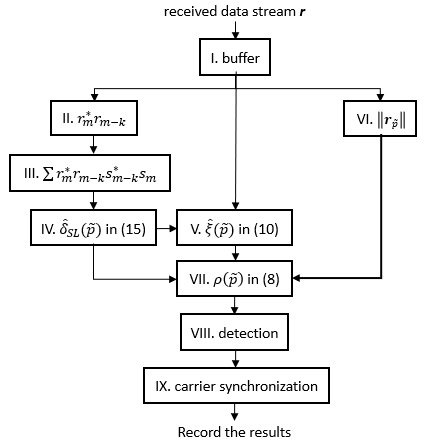
\includegraphics[width=2.7in,height=2.6in]{SDR_receiver_new.png}}
    \caption{Block diagram for implementing the proposed algorithm in TBB}
    \label{fig:SDR_receiver}
    \end{figure}

% To make our proposed algorithm work at a very high sample rate,
% the first improvement of algorithm is by using pipeline.
% Threading Building Blocks (TBB) is a well-known C++
% library that enables parallel programming on multicore processor~\cite{Michael_19}.
To demonstrate the practicality of our algorithms, we have implemented them in C++ on a general
purpose processor (GPP).
The different aspects of the algorithm are mapped to logical nodes in a pipelined, parallel processing architecture
using Threading Building Blocks (TBB)~\cite{Michael_19}.

Figure~\ref{fig:SDR_receiver} shows a simple block diagram
illustrating the pipeline for the complete joint detection and
estimation process.
Due to space constraints, we cannot give details for each node; the
computations performed by the nodes relate closely to the expressions
throughout this paper some of which are indicated in Figure~\ref{fig:SDR_receiver}.

It is necessary to discuss the node for computing the phasor estimate $\hat{\xi}$ (node V). 
The numerator of~\eqref{eq:opt_xi} performs a time-varying
convolution,
which cannot be computed efficiently via FFT.
Our solution to increasing the computational efficiency is to further
parallelize this block.
Specifically,~\eqref{eq:opt_xi} can be computed in three stages:
1.~Compute  segments of $\sum r_ns_n^*$ in  parallel;
2.~still in parallel, each segment is then phase-shifted by $\hat{\delta}_{SL}$
multiplied by the middle index of the 
segment.
3. Sum all segments together.
In other words, \eqref{eq:opt_xi} is computed more efficiently as
\begin{equation}
  \label{eq:refined_opt_S}
  ||\bm{s}||^2\cdot\hat{\xi} \approx \sum_{i=0}^{L-1} e^{-j\pi \hat{\delta}\frac{N(2i+1)}{L}}
  \sum_{n=iN/L}^{(i+1)N/L-1}r_ns_n^*,
\end{equation}
where $L$ is the number of segments processed in parallel.
As a result,
the efficiency of computing $\hat{\xi}$ is improved by $L^2$.

We now show the results of implementing the proposed algorithm on SDR
by using
highly parallel execution on SDR.
The signals are transmitted and received between two universal software radio peripherals (USRP);
these are connected by \SI[per-mode=symbol]{5}{\giga\bits\per\second} Ethernet cables to
laptops.
On the receiver side, 
the CPU includes 6 cores and 12 threads with a \SI{4.5}{\giga\hertz}
clock frequency.

Each node in Figure~\ref{fig:SDR_receiver} was benchmarked (using Google benchmark) to measure their throughput.
The results for each node are shown 
in Table~\ref{table:BM_function_nodes}.
Note, that the times displayed in the table
refers to processing a  buffer of size 8192 samples.
The throughput of the 
pipeline is dominated by the node with the longest execution time.
Thus, the  throughput of our current implementation is bounded by
$\SI{8192}{\sample}/\SI{837253}{\nano\second}  \approx \SI[per-mode=symbol]{9.78}{\mega\sample\per\second}$.
In operation, the throughput of the algorithm was measured to be in
the range of
\SI[per-mode=symbol]{4.5}{\mega\sample\per\second} to \SI[per-mode=symbol]{5}{\mega\sample\per\second} with latency near \SI{1}{\milli\second}.
The detection algorithm is very robust and the false alarm probability is near 0 at moderate SNR.

\begin{table}[t]
    \caption{Benchmark results of nodes in Figure~\ref{fig:SDR_receiver} with buffer size 8192}  % title of Table
    \centering % used for centering table
    \begin{tabular}{c c c c} % centered columns (4 columns)
    \hline\hline %inserts double horizontal lines
    Node name & Time (ns) & CPU (ns) & Iterations \\ [0.5ex] % inserts table
    %heading
    \hline % inserts single horizontal line
    I. Buffer  & 408721 & 407754 & 1703 \\ % inserting body of the table
    II. $r_m^*r_{m-k}$  & 160069 & 160054 & 3416 \\
    III. $r_m^*r_{m-k}s_{m-k}^*s_m$ & 498967 & 498876 & 1471 \\
    IV. $\hat{\delta}_{SL}^{(1)}$ & 187135 & 187121 & 3602 \\
    V. $\hat{\xi}$ & 780620 & 780523 & 886 \\
    VI. $||\bm{r}||$ & 203907 & 203892 & 3416 \\ % [1ex] adds vertical space
    VII. $\rho(p)$ & 837253 & 837048 & 829 \\
    VIII. detection & 378793 & 378765 & 1844 \\
    IX. carrier synchronization & 811747 & 811739 & 844  \\ [1ex]
    \hline
    \end{tabular}
    \label{table:BM_function_nodes} % is used to refer this table in the text
  \end{table}

